\documentclass[10pt]{article}
\usepackage{hyperref}
\usepackage{amsmath}
\usepackage{amsfonts}
\usepackage{minted}
\usepackage{tikz}
\usetikzlibrary{arrows,backgrounds,shapes,matrix,positioning,fit,calc}
\usetikzlibrary{decorations.pathreplacing,angles,quotes}
\usetikzlibrary{arrows.meta}
\usetikzlibrary{calendar}
\usetikzlibrary{trees}


\title{MiMC in Halo2}
\date{}
\author{}

\begin{document}
\maketitle
\begin{abstract}
  We give a specification of the MiMC block ciphers for implementation in the Pasta elliptic curve fields. The specification closely follows the MiMC implementation in \texttt{circom}. We also outline the proposed implementation strategy in Halo2.
\end{abstract}
  
\section{Introduction}%
\label{sec:introduction}
The MiMC block ciphers were designed to have low multiplicative complexity \cite{cryptoeprint:2016/492}. Two variants were proposed: one based on a cubic round function and the other having a Feistel network structure (with a cubic round function). We will refer to them as \texttt{MiMC} and \texttt{MiMC-Feistel} for convenience. The MiMC hash functions are obtained from these block ciphers by setting the key value to zero.

We are interested in MiMC implementations when the input, output, and key are from a prime field $\mathbb{F}_p$.
\subsection{\texttt{MiMC} over  a prime field}%
\label{subsec:mimc_over_a_prime_field_}


A \texttt{MiMC} block cipher implementation over $\mathbb{F}_p$ is specified as below:
\begin{itemize}
  \item Set $s$ to be smallest integer greater than one that satisfies $\gcd(s, p-1)=1$. The gcd condition ensures that $x^s$ is a permutation in $\mathbb{F}_p$. We want $s$ to be the smallest such integer to keep the multiplicative complexity minimal.
  \item The cipher has $r$ rounds where $r = \left\lceil \frac{\log_2 p}{\log_2 s}  \right\rceil$.
  \item Let $\{c_i \in \mathbb{F}_p \mid i=0,1,\ldots,r-1 \}$ be the $r$ round constants. By convention, the first round constant is set to zero, i.e.~$c_0= 0$. The remaining round constants are derived in a pseudorandom manner and are fixed for a particular implementation.
  \item The $i$th round function is given by $F_i(x) = (x + k + c_i)^s$ where $k \in \mathbb{F}_p$ is the secret key.
  \item The encryption of $x \in \mathbb{F}_p$ is given by
    \begin{align*}
      E_k(x) & = F_{r-1}(\cdots F_2(F_1(F_0(x))) \cdots) + k\\
             & = \left(\cdots \left((x+k+c_0)^s + k + c_1\right)^s \cdots + k + c_{r-1}\right)^s + k.
    \end{align*}
    This is illustrated in Figure \ref{fig:MiMCEncryption}.
\end{itemize}
\begin{figure}[t]
\begin{center}
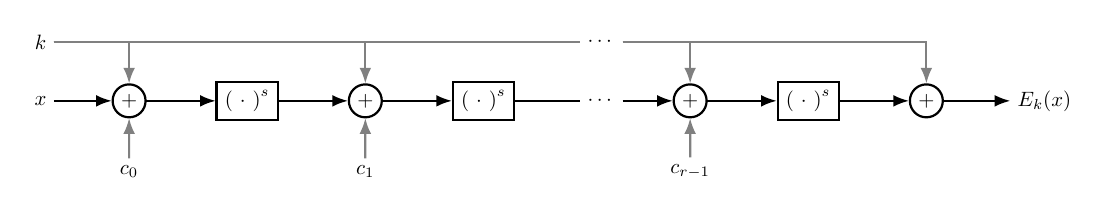
\begin{tikzpicture}[scale=0.75, transform shape]
  \node at (-0.5, 0) (x) {$x$};
  \node at (-0.5, 1) (k) {$k$};
  \node[draw, thick, circle, inner sep=2pt] at (1.0, 0) (add0) {$+$};
  \node at (1.0, -1.2) (c0) {$c_0$};
  \node[draw, thick, rectangle, inner sep=4pt] at (3.0, 0) (power0) {$\left( \ \cdot \  \right)^s$};
  \node[draw, thick, circle, inner sep=2pt] at (5.0, 0) (add1) {$+$};
  \node at (5.0, -1.2) (c1) {$c_1$};
  \node[draw, thick, rectangle, inner sep=4pt] at (7.0, 0) (power1) {$\left( \ \cdot \  \right)^s$};
  \node at (9, 0) (dots0) {$\cdots$};
  \node at (9, 1) (dots1) {$\cdots$};
  \node[draw, thick, circle, inner sep=2pt] at (10.5, 0) (addr1) {$+$};
  \node at (10.5, -1.2) (cr1) {$c_{r-1}$};
  \node[draw, thick, rectangle, inner sep=4pt] at (12.5, 0) (powerr1) {$\left( \ \cdot \  \right)^s$};
  \node[draw, thick, circle, inner sep=2pt] at (14.5, 0) (addr) {$+$};
  \node at (16.5, 0) (Ek) {$E_k(x)$};

  \draw[gray, thick,-{Latex[length=2mm]}] (k) -| (add0.north);
  \draw[gray, thick,-{Latex[length=2mm]}] (k) -| (add1.north);
  \draw[gray, thick] (k) -- (dots1);
  \draw[gray, thick,-{Latex[length=2mm]}] (dots1) -| (addr1.north);
  \draw[gray, thick,-{Latex[length=2mm]}] (dots1) -| (addr.north);

  \draw[thick,-{Latex[length=2mm]}] (x) -- (add0.west);
  \draw[gray,thick,-{Latex[length=2mm]}] (c0) -- (add0.south);
  \draw[thick,-{Latex[length=2mm]}] (add0.east) -- (power0);
  \draw[thick,-{Latex[length=2mm]}] (power0) -- (add1.west);
  \draw[gray,thick,-{Latex[length=2mm]}] (c1) -- (add1.south);
  \draw[thick,-{Latex[length=2mm]}] (add1.east) -- (power1);
  \draw[thick] (power1) -- (dots0);
  \draw[thick,-{Latex[length=2mm]}] (dots0) -- (addr1);
  \draw[gray,thick,-{Latex[length=2mm]}] (cr1) -- (addr1.south);
  \draw[thick,-{Latex[length=2mm]}] (addr1) -- (powerr1);
  \draw[thick,-{Latex[length=2mm]}] (powerr1) -- (addr);
  \draw[thick,-{Latex[length=2mm]}] (addr) -- (Ek);
\end{tikzpicture}
\end{center}
\caption{\texttt{MiMC} Encryption}%
\label{fig:MiMCEncryption}
\end{figure}

\subsection{\texttt{MiMC-Feistel} over a prime field}%
\label{subsec:mimc-feistel_over_a_prime_field}


A \texttt{MiMC-Feistel} implementation over $\mathbb{F}_p$ is specified as below:
\begin{itemize}
  \item Once again, set $s$ to be smallest integer greater than one that satisfies $\gcd(s, p-1)=1$.
  \item The cipher has $r$ rounds where $r = 2\times\left\lceil \frac{\log_2 p}{\log_2 s}  \right\rceil$. Note that the number of rounds is twice as large as the number used in \texttt{MiMC}.
  \item Let $\{c_i \in \mathbb{F}_p \mid i=0,1,\ldots,r-1 \}$ be the $r$ round constants. By convention, the first and last round constants are set to zero, i.e.~$c_0=c_{r-1} = 0$. The remaining round constants are derived in a pseudorandom manner and are fixed for a particular implementation.
  \item In the first $r-1$ rounds, the $i$th round function is given by 
    \begin{align*}
    F_i(x_L \| x_R)  =  \left( x_R + \left( x_L+k+c_i\right)^s  \right) \| x_L, \quad i=0,1,\ldots,r-1,
    \end{align*}
    where $x_L, x_R \in \mathbb{F}_p$ are the inputs and $k \in \mathbb{F}_p$ is the secret key.
  \item The last round function is given by
    \begin{align*}
    F_{r-1}(x_L \| x_R) =  x_L\| \left( x_R + \left( x_L+k+c_{r-1}\right)^s \right).
    \end{align*}
    It does not perform the swap operation seen in previous rounds.
  \item The encryption of $x_L \| x_R \in \mathbb{F}_p^2$ is given by
    \begin{align*}
      E_k(x) & = F_{r-1}(\cdots F_2(F_1(F_0(x_L \| x_R))) \cdots).
    \end{align*}
    This is illustrated in Figure \ref{fig:MiMCFeistelEncryption}.
\end{itemize}

\begin{figure}[t]
\begin{center}
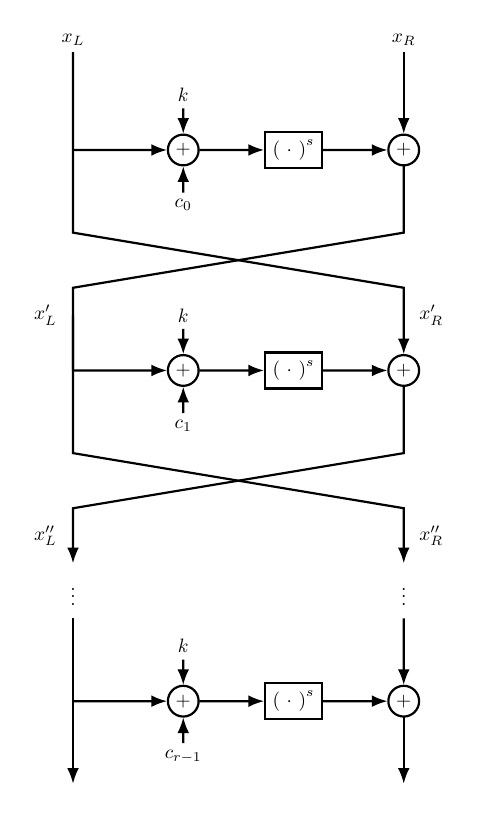
\begin{tikzpicture}[scale=0.70, transform shape]
  \node at (0,10) (xL) {$x_L$};
  \node at (6,10) (xR) {$x_R$};
  \node at (2,9.0) (k0) {$k$};
  \node at (2,7.0) (c0) {$c_0$};
  \node[draw, thick, circle, inner sep=2pt] at (2,8) (add0mid) {$+$};
  \node[draw, thick, circle, inner sep=2pt] at (6,8) (add0right) {$+$};
  \node[draw, thick, rectangle, inner sep=4pt] at (4, 8) (power0) {$\left( \ \cdot \  \right)^s$};

  \node at (-0.5,5.0) (xLprime) {$x_L'$};
  \node at (6.5,5.0) (xRprime) {$x_R'$};
  \node at (2,5.0) (k1) {$k$};
  \node at (2,3.0) (c1) {$c_1$};
  \node[draw, thick, circle, inner sep=2pt] at (2,4) (add1mid) {$+$};
  \node[draw, thick, circle, inner sep=2pt] at (6,4) (add1right) {$+$};
  \node[draw, thick, rectangle, inner sep=4pt] at (4,4) (power1) {$\left( \ \cdot \  \right)^s$};

  \draw[thick,-{Latex[length=2mm]}] (xL) -- ($(xL)+(0,-3.5)$) -- ($(xR)+(0,-4.5)$) -- (add1right.north);
  \draw[thick] (add0right.south) -- ($(xR)+(0,-3.5)$) -- ($(xL)+(0,-4.5)$)-- ($(xL)+(0,-6.0)$);
  \draw[thick,-{Latex[length=2mm]}] (k0) -- (add0mid);
  \draw[thick,-{Latex[length=2mm]}] (c0) -- (add0mid);
  \draw[thick,-{Latex[length=2mm]}] (xR) -- (add0right);
  \draw[thick,-{Latex[length=2mm]}] (add0mid) -- (power0);
  \draw[thick,-{Latex[length=2mm]}] (power0) -- (add0right);
  \draw[thick,-{Latex[length=2mm]}] (0,8) -- (add0mid);

  \draw[thick,-{Latex[length=2mm]}] ($(xL)+(0,-5.0)$) -- ($(xL)+(0,-7.5)$)-- ($(xR)+(0,-8.5)$)-- ($(xR)+(0,-9.5)$);
  \draw[thick,-{Latex[length=2mm]}] (add1right.south) -- ($(xR)+(0,-7.5)$) -- ($(xL)+(0,-8.5)$)-- ($(xL)+(0,-9.5)$);
  \draw[thick,-{Latex[length=2mm]}] (k1) -- (add1mid);
  \draw[thick,-{Latex[length=2mm]}] (c1) -- (add1mid);
  \draw[thick,-{Latex[length=2mm]}] (add1mid) -- (power1);
  \draw[thick,-{Latex[length=2mm]}] (power1) -- (add1right);
  \draw[thick,-{Latex[length=2mm]}] (0,4) -- (add1mid);


  \node at ($(xL)+(-0.5,-9)$) (xLprimeprime) {$x_L''$};
  \node at ($(xR)+(0.5,-9)$) (xRprimeprime) {$x_R''$};
  \node at ($(xL)+(0,-10)$) (vdotsL) {$\vdots$};
  \node at ($(xR)+(0,-10)$) (vdotsR) {$\vdots$};
  \node at (2,-1.0) (kr1) {$k$};
  \node at (2,-3.0) (cr1) {$c_{r-1}$};
  \node[draw, thick, circle, inner sep=2pt] at (2,-2) (addr1mid) {$+$};
  \node[draw, thick, circle, inner sep=2pt] at (6,-2) (addr1right) {$+$};
  \node[draw, thick, rectangle, inner sep=4pt] at (4, -2) (powerr1) {$\left( \ \cdot \  \right)^s$};

  \draw[thick,-{Latex[length=2mm]}] ($(vdotsL)+(0,-0.5)$) -- ($(xL)+(0,-13.5)$);
  \draw[thick,-{Latex[length=2mm]}] (addr1right.south) -- ($(xR)+(0,-13.5)$);
  \draw[thick,-{Latex[length=2mm]}] (kr1) -- (addr1mid);
  \draw[thick,-{Latex[length=2mm]}] (cr1) -- (addr1mid);
  \draw[thick,-{Latex[length=2mm]}] (addr1mid) -- (powerr1);
  \draw[thick,-{Latex[length=2mm]}] (powerr1) -- (addr1right);
  \draw[thick,-{Latex[length=2mm]}] (0,-2) -- (addr1mid);
  \draw[thick,-{Latex[length=2mm]}] ($(vdotsR)+(0,-0.5)$) -- (addr1right);

\end{tikzpicture}
\end{center}
\caption{\texttt{MiMC} Feistel Encryption}%
\label{fig:MiMCFeistelEncryption}
\end{figure}


\section{MiMC in \texttt{circom}}%
\label{sec:mimc_in_circom}
The \texttt{circom} library \cite{circomlib} has implementations of both \texttt{MiMC} and \texttt{MiMC-Feistel} ciphers. The \texttt{MiMC} implementation in \texttt{circom} uses $s=7$ while the \texttt{MiMC-Feistel} implementation uses $s=5$.\footnote{
It is not clear why $s=7$ was chosen for \texttt{MiMC} in \texttt{circom}. The field where the MiMC calculations will occur has order equal to the group order of the alt\textunderscore bn128 (BN254) curve. This order is given by the prime
\begin{align*}
{\scriptstyle
  p\  =\  21888242871839275222246405745257275088548364400416034343698204186575808495617.
}
\end{align*}
While $\gcd(p-1, 3) = 3$, we have $\gcd(p-1, 5)=1$. So $s=5$ is a valid choice. In a document describing EdDSA on the Baby Jubjub curve \cite{eddsa_babyjubjub_mimc7}, the authors mention that $s=7$ is the optimal choice since $\gcd(l-1, 3)=3$ where $l$ is group order of the Baby Jubjub curve. It turns out that $\gcd(l-1, 5)=5$ and $\gcd(l-1, 7)=1$. But the order of elliptic curve group should not matter.
}

The \texttt{MiMC} implementation has 91 rounds where the round constants are elements in $\mathbb{F}_p$ where $p$ is the order of the alt\textunderscore bn128 curve. Figure \ref{fig:MiMCconstantscircom} shows pseudocode of the round constant calculation.\footnote{See \url{https://github.com/iden3/circomlibjs/blob/main/src/mimc7.js} for a Javascript implementation of the round constant calculation.} It hashes the string ``mimc'' iteratively using the Keccak256 hash function and converts the resulting value into a field element in $\mathbb{F}_p$. By convention, the first round constant is set to zero.
\begin{figure}[t]
\begin{minted}[fontsize=\scriptsize]{python}
prime = 21888242871839275222246405745257275088548364400416034343698204186575808495617
num_rounds = ceil(log(prime,2)/log(7,2))

SEED = "mimc"
hash_val = keccak256(SEED)

F = GF(prime)
round_constants[0] = F(0)

for i in range(1, num_rounds):
      hash_val = keccak256(hash_val)
      round_constants[i] = F(hash_val)
\end{minted}
\caption{\texttt{MiMC} round constant generation in \texttt{circom}}%
\label{fig:MiMCconstantscircom}
\end{figure}

The \texttt{MiMC-Feistel} implementation in \texttt{circom} has 220 rounds. The pseudocode for the round constant calculation is shown in Figure \ref{fig:MiMCFeistelconstantscircom}. The number of rounds is calculated assuming $s=5$ and the seed string is chosen to be ``mimcsponge''. By convention, the first and last round constants are set to zero.

\begin{figure}[t]
\begin{minted}[fontsize=\scriptsize]{python}
prime = 21888242871839275222246405745257275088548364400416034343698204186575808495617
num_rounds = 2*ceil(log(prime,2)/log(5,2))

SEED = "mimcsponge"
hash_val = keccak256(SEED)

F = GF(prime)
round_constants[0] = F(0)
round_constants[num_rounds-1] = F(0)

for i in range(1, num_rounds-1):
      hash_val = keccak256(hash_val)
      round_constants[i] = F(hash_val)
\end{minted}
\caption{\texttt{MiMC-Feistel} round constant generation in \texttt{circom}}%
\label{fig:MiMCFeistelconstantscircom}
\end{figure}

\section{MiMC in Pasta Fields}%
\label{sec:mimc_in_halo2}
Halo2 has a pair of elliptic curves called Pallas and Vesta. For
\begin{align*}
  p & = \texttt{0x40000000000000000000000000000000224698fc094cf91b992d30ed00000001},\\
  q & = \texttt{0x40000000000000000000000000000000224698fc0994a8dd8c46eb2100000001},
\end{align*}
the Pallas curve is given by the equation $y^2 = x^3+5$ over $\mathbb{F}_p$. It forms a group of order $q$. The Vesta curve is given by the same equation over $\mathbb{F}_q$ and it forms a group of order $p$.

Since $\gcd(p-1, 3) = \gcd(q-1, 3) = 3$ and $\gcd(p-1, 5)=\gcd(q-1, 5)=1$, we propose to use $s=5$ in the Halo2 MiMC implementations.

The number of \texttt{MiMC} rounds in both Pasta fields will be 110, as $\left\lceil \frac{\log_2 p}{\log_2 5} \right\rceil = \left\lceil \frac{\log_2 q}{\log_2 5} \right\rceil = 110$. And the number of \texttt{MiMC-Feistel} rounds will be 220.
\subsection{Round Constant Generation}%
\label{subsec:round_constant_generation}
We propose to use the same algorithm as \texttt{circom} to generate round constants (with the Pasta fields substituted for the alt\textunderscore bn128 scalar field).

Sage codes for generating the Pallas field round constants for \texttt{MiMC} and \texttt{MiMC-Feistel} are given in Appendix \ref{sec:mimc_constant_generation_for_pallas} and Appendix \ref{sec:mimc_feistel_constant_generation_for_pallas}. These programs and the generated constants are available at \url{https://github.com/avras/pasta-mimc}.

\section{MiMC implementation in Halo2}%
\label{sec:mimc_implementation_in_halo2}

\subsection{\texttt{MiMC} in Halo2}%
\label{subsec:mimc_in_halo2}
Columns
\begin{itemize}
  \item One instance column to hold the input $x$, key $k$, and output $E_k(x)$ at offsets 0, 1, and 2
  \item One fixed column to hold the round constants; the $i$th row holds $c_i$
  \item One advice column where $i$th row holds $y_i$ where
    \begin{align*}
      y_i = 
      \begin{cases}
        x & \text{ if } i = 0,\\
        (y_{i-1} + k + c_{i-1})^5 & \text{ if } 1 \le i \le  110,\\
        y_{i-1} + k & \text{ if } i=111.
      \end{cases}
    \end{align*}
  \item Three selectors: $s_1,s_2,s_3$
    \begin{align*}
      s_1 = 1 & \iff i=0\\
      s_2 = 1 & \iff 1 \le i\le 110\\
      s_3 = 1 & \iff i=111
    \end{align*}
\end{itemize}

\subsection{\texttt{MiMC-Feistel} in Halo2}%
\label{subsec:mimc_feistel_in_halo2}
Columns
\begin{itemize}
  \item One instance column to hold the inputs $x_L, x_R$, key $k$, and output $E_k(x)$ at offsets 0, 1, 2, and 3
  \item One fixed column to hold the round constants; the $i$th row holds $c_i$
  \item Two advice columns whose $i$th rows hold $y_i$ and $z_i$ where
    \begin{align*}
      y_i \| z_i = 
      \begin{cases}
        x_L \| x_R & \text{ if } i = 0,\\
        \left( z_{i-1} + \left( y_{i-1}+k+c_{i-1}\right)^5  \right) \bigg\| y_{i-1} & \text{ if } 1 \le i \le  219,\\
        y_{i-1} \bigg\| \left( z_{i-1} + \left( y_{i-1}+k\right)^5  \right) & \text{ if } i=220.
      \end{cases}
    \end{align*}
  \item Three selectors: $s_1,s_2,s_3$
    \begin{align*}
      s_1 = 1 & \iff i=0\\
      s_2 = 1 & \iff 1 \le i\le 219\\
      s_3 = 1 & \iff i=220
    \end{align*}
\end{itemize}






\newpage
\appendix
\section{\texttt{MiMC} constant generation for Pallas field}%
\label{sec:mimc_constant_generation_for_pallas}
\begin{minted}{python}
from sage.all import *
from Crypto.Hash import keccak

prime = 0x40000000000000000000000000000000224698fc094cf91b992d30ed00000001
num_rounds = ceil(log(prime,2)/log(5,2))
print('Number of rounds =', num_rounds)

F = GF(prime)
round_constants = [F(0)]

seed_value = b'mimc';
keccak_hash = keccak.new(data=seed_value, digest_bits=256)
hash_val = keccak_hash.digest()

for i in range(1,num_rounds):
    keccak_hash = keccak.new(data=hash_val, digest_bits=256)
    hash_val = keccak_hash.digest()
    hash_val_in_hex = keccak_hash.hexdigest()

    field_element = F('0x'+hash_val_in_hex)
    round_constants.append(field_element)

print ('round_constants = [')
for i in range(num_rounds):
    print('   ', hex(round_constants[i])+',')
print(']')
\end{minted}

\newpage
\section{\texttt{MiMC-Feistel} constant generation for Pallas field}%
\label{sec:mimc_feistel_constant_generation_for_pallas}
\begin{minted}{python}
from sage.all import *
from Crypto.Hash import keccak

prime = 0x40000000000000000000000000000000224698fc094cf91b992d30ed00000001
num_rounds = 2*ceil(log(prime,2)/log(5,2))
print('Number of rounds =', num_rounds)

F = GF(prime)
round_constants = [F(0)]

seed_value = b'mimcsponge';
keccak_hash = keccak.new(data=seed_value, digest_bits=256)
hash_val = keccak_hash.digest()

for i in range(1,num_rounds-1):
    keccak_hash = keccak.new(data=hash_val, digest_bits=256)
    hash_val = keccak_hash.digest()
    hash_val_in_hex = keccak_hash.hexdigest()

    field_element = F('0x'+hash_val_in_hex)
    round_constants.append(field_element)
round_constants.append(F(0))

print ('round_constants = [')
for i in range(num_rounds):
    print('   ', hex(round_constants[i])+',')
print(']')
\end{minted}


\newpage
\bibliographystyle{unsrt}
\bibliography{mimc}
\end{document}
